\section{Related Work}
This section should summarise all the research you have completed so far, e.g. previous products and research papers. You should start with a broad summary and then become more focused in the sub-sections, as appropriate. For example, you might be doing a VR project for use in a museum. You first want to summarise what VR is and some example uses, then identify any previous work in a museum. Sub-sections might be ``VR for museum tours'' and ``VR design practices''. Then your research questions could be that you have identified shortfalls in the tours because they have not been designed with museums in mind from the outset. Therefore you questions will be around identifying value from a new tour design. 

\subsection{Related Work Focus 1}

\begin{figure}
\centering
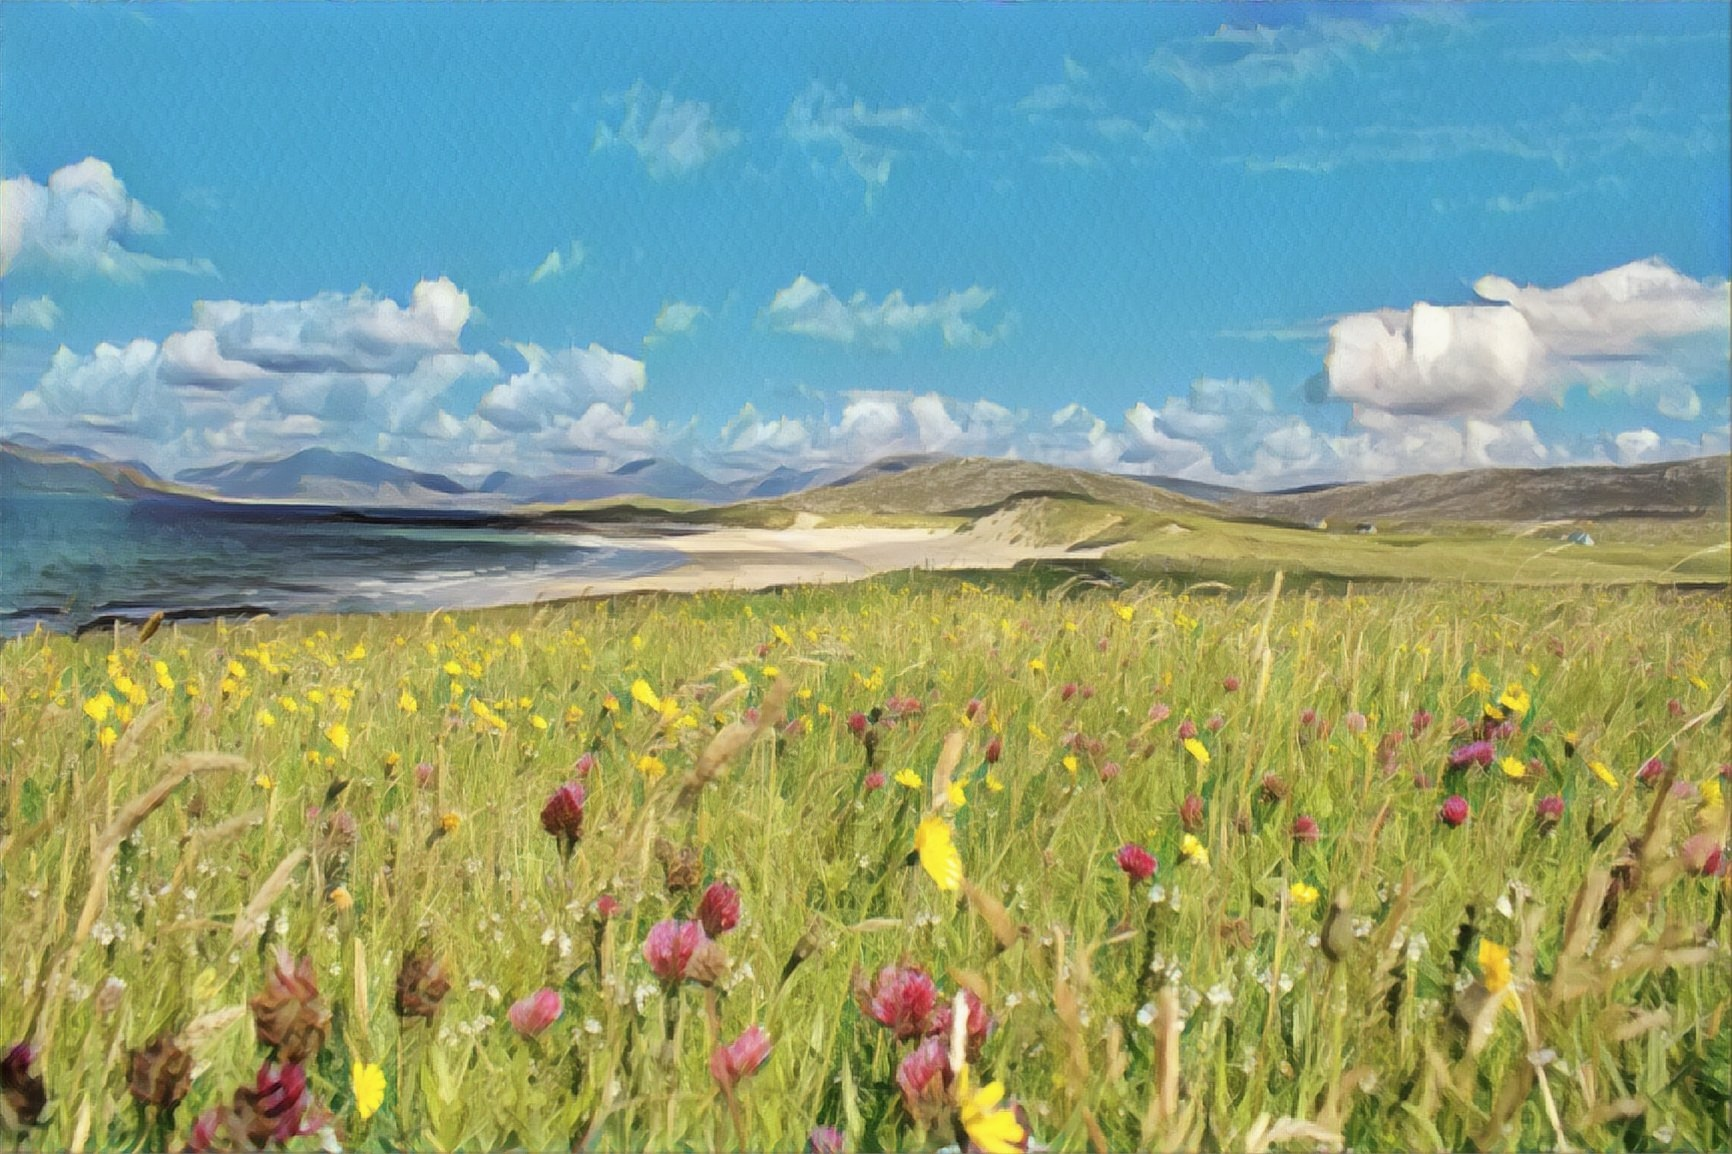
\includegraphics[width=1\columnwidth]{author-files/figures/scarista.jpg}
\caption{Painting of Scarista}
\label{fig:scarista}
\end{figure}

\lipsum[20]

\subsection{Related Work - Focus 2}

You may wish to include tables such as Table \ref{tab:freq} in your report. You can either google how to manually create a table or you can create one using this link: \url{https://www.tablesgenerator.com/}


\begin{table}
  \caption{Hokey Information}
  \label{tab:freq}
  \begin{tabular}{ccl}
    \toprule
    Location&Frequency&Comments\\
    \midrule
    In & 1 in 1,000& Very much in\\
    Out & 1 in 5& Very much out\\
    Shaken Aboot & 4 in 5 & Not stirred\\
  \bottomrule
\end{tabular}
\end{table}


\subsection{Research Questions and / or Aims}
If you are doing a purely software development project you should use this section to identify clearly the gap that you have found in your previous research and outline how your new system will address this. 

If you are doing a project with a research focus, then you should identify clearly the gap that you have found and outline your research questions:
\begin{itemize}
    \item [RQ1] How much wood would a wood chuck chuck if a wood chuck could chuck wood?
    \item [RQ2] How much wood would a wood chuck chuck if a wood chuck could chuck wood?
\end{itemize}

